%ustawienia
\documentclass[12pt,a4paper]{article}
\usepackage[T1]{fontenc}
\usepackage{mathptmx}
\usepackage[utf8]{inputenc}
\usepackage{amssymb}
\usepackage[polish]{babel}
\usepackage{polski}
\usepackage{amsmath}
\usepackage{amsfonts}
\usepackage[left=3.5cm,right=2cm,top=2.5cm,bottom=2.5cm]{geometry}
\usepackage{graphicx}
\usepackage{indentfirst} 
\usepackage{float}
\usepackage{hyperref}
\usepackage[most]{tcolorbox}
\setlength{\parindent}{0.7cm}
\hypersetup{
	colorlinks = true,
	linkcolor = black,
	filecolor = magenta,
	urlcolor = blue,
	}
\urlstyle{same}	
	
\author{Karpiński Maciej\\Radlak Piotr\\Wiecheć Sebastian\\\\\\\\\includegraphics[width=0.7\linewidth]{img/logoPWSZ.eps}\\\\\\\\Projektowanie i programowanie systemów internetowych I}
\title{Projekt systemu zleceń mafijnych\\,,Mafia 2.0''}

\begin{document}

	%Stron tytułowa
	\maketitle
	\thispagestyle{empty}
	\pagenumbering{arabic} 
	\clearpage

	%Spis treści
	\tableofcontents
	\newpage

	%Początek pierwszej sekcji opisującej system
	\section{Opis funkcjonalny systemu}
		\indent System zleceń mafijnych ,,Mafia 2.0'' jest aplikacją internetową pozwalającą zarejestrowanemu i zalogowanemu użytkownikowi na przeglądanie i składanie zleceń,
		wykonywanych przez zorganizowane grupy przestępcze. Funkcjonalność aplikacji obejmuje:
		\begin{itemize}
			\item dostęp do aplikacji poprzez przeglądarkę www (PC, smartphone),
			\item rejestrację i logowanie użytkowników,
			\item przeglądanie oferty zleceń,
			\item wysłania e-maila do użytkownika z potwierdzeniem rejestracji/zlecenia,
			\item wyświetlenie aktualnego kursu Franka Szwajcarskiego (CHF),
			\item Polską i Angielską lokalizacje;
		\end{itemize}
	\newpage

	%Sekcja druga, opis wdrożonych kwalifikacji
	\section{Wdrożone kwalifikacje}	
		\indent Aplikacja została stworzona na bazie frameworku aplikacji webowych ASP .NET Core i~opartej na wzorcu Model-View-Controller(MVC), posiada wbudowany router oraz wykorzystuje
		silnik Razer do dynamicznego generowania wysyłanych plików HTML.
		Do zarządzania zależnościami w projekcie wykorzystaliśmy menadżer pakietów NuGet.
		Wykorzystanie w projekcie Bootstrapa zapewnia ostylowanie i RWD frontendu aplikacji internetowej ,,Mafia 2.0''.
		Użytkownik przy pomocy formularzy posiada możliwość rejestracji, logowania i przesyłania innych danych do aplikacji.
		Do komunikacji z zewnętrzną bazą danych Microsoft SQL Server, został wykorzystany EntityFramework, który zapewnia system mapowania relacyjno-obiektowego (ORM)
		oraz umożliwia dodawanie, usuwanie i~edycję rekordów w~bazie danych.
		Poprzez zastosowaniu pakietu MailKit można z poziomu aplikacji łączyć się z serwerem pocztowym i wysyłać e-maile.
		System zleceń mafijnych ,,Mafia 2.0'' wykorzystuje zewnętrzne API w celu pobrania aktualnego kursu Franka Szwajcarskiego, dodatkowo aplikacji wystawia API z danymi
		dotyczącymi wykonywanych zleceń.
		Każda akcja wykonująca działanie na bazie danych jest zapisywana.
		W ramach optymalizacji SEO została uruchomiona kompresja gzip na reverse proxy NGINX dodatkowo dzięki użyciu pakietu Grunt zautomatyzowano mimifikację JavaScript i CSS.
		Wszystkie statyczne pliki (.css, .js, .png, .jpg, .gif, .svg) mają ustawiony cache na 365 dni oraz dodatkowo wystawiają wersję kontrolną, dzięki czemu w~przypadku zmiany na serwerze
		przeglądarka może pobrać nową wersję pliku przed upływem określonego czasu. Aplikacja jest zlokalizowana w języku polskim i~angielskim.
	\newpage

	%sekcja trzecia, opis wykorzystanych technologii
	\section{Opis technologiczny}
		\indent Przy tworzeniu projektu ,,Mafia 2.0'' wykorzystano następujące technologie:

		\subsection{C\#}
			\indent C\# jest obiektowym językiem programowania, zaprojektowanym w latach 1998 – 2001 dla firmy Microsoft.
			Napisany program jest kompilowany do Common Intermediate Language(CLI), który następnie wykonywany jest w środowisku uruchomieniowym takim jak .NET Framework,
			.NET Core, Mono lub DotGNU.
			Wykorzystanie CLI sprawia, że kod programu jest wieleplatformowy (dopóki istnieje odpowiednie środowisko uruchomieniowe).
			C\# posiada wiele wspólnych cech z językami Object Pascal, Delphi, C++ i Java a najważniejszymi cechami C\# są:
			\begin{itemize}
				\item Obiektowość z hierarchią o jednym elemencie nadrzędnym (podobnie jak w Javie);
				\item Zarządzaniem pamięcią zajmuje się środowisko uruchomieniowe;
				\item Właściwości i indeksery;
				\item Delegaty i zdarzenia – rozwinięcie wskaźników C++;
				\item Typy ogólne, generyczne, częściowe, Nullable, domniemane, anonimowe;
				\item Dynamiczne tworzenie kodu;
				\item Metody anonimowe;
				\item Wyrażenia lambda.
			\end{itemize}
			
		\subsection{ASP.NET Core 3.1}
			\indent ASP.Net Core jest wysokowydajnym frameworkiem, do budowania nowoczesnych aplikacji internetowych wykorzystujących moc obliczeniową chmur. ASP.Net Core jest technologią
			open - source, wykorzystującą silnik html Razor, dzięki której możliwe jest tworzenie aplikacji mulitplaformowych, które mogą być używane na każdym urządzeniu wyposażonym
			w przeglądarkę internetową.
			
		\subsection{Bootstrap}		
			\indent Bootstrap jest frameworkiem CSS, który koncentruje się na uproszczeniu tworzenia frontendu stron internetowych. Rezultatem dodania Bootstrapa do projektu jest
			jednolity wygląd wszystkich elementów interfejsów we wszystkich przeglądarkach. Dodatkowo programiści mogą skorzystać z klas w CSS w celu dalszego dostosowywania
			wyglądu ich zawartości. Bootstrap zawiera kilka składników JavaScript, które zapewniają dodatkowe elementy interfejsu użytkownika, takie jak okna dialogowe, podpowiedzi
			czy karuzele. 

		\subsection{Entity Framework}		 
		 	\indent Entity Framework jest technologią open - source do mapowania obiektowo – relacyjnego (ORM), które wspierają rozwój aplikacji zorientowanych na dane.
		 	Entity Framework umożliwia programistom pracę z danymi w postaci obiektów i właściwości specyficznych dla domeny, bez konieczności przejmowania się bazowymi
		 	tabelami i kolumnami baz danych, w których dane są przechowywane. 

		\subsection{Microsoft SQL Server}		 
		 	\indent Microsoft SQL Server jest systemem zarządzania relacyjnymi bazami danych opracowany przez firmę Microsoft. Cechą charakterystyczną jest głównie wykorzystywanie języka
		 	zapytań	Transact-SQL, który jest rozwinięciem standardu ANSI/ISO. W projekcie wykorzystano wersje 2019 Express, która jest bezpłatną edycją programu Microsoft SQL Server, oferująca
		 	podstawowy silnik bazy danych, nieposiadający ograniczenia ilości obsługiwanych baz lub użytkowników. Ograniczenia, występujące w wersji Express to  m.in.:
		 	korzystanie z~jednego procesora, 1 GB pamięci RAM, 10GB plików bazy danych czy brak SQL Agent.
		
		\subsection{MailKit}
			\indent MailKit jest multiplatformową otwarto źródłową biblioteką .NET klienta pocztowego opartą o MimeKit, która została zoptymalizowana pod kątem urządzeń mobilnych.
			MailKit oferuje następującą funkcjonalność:
			\begin{itemize}
				\item Obsługa proxy HTTP, Socks4, Socks4a i Socks5;
				\item Uwierzytelnianie SASL;
				\item Kompletny klient SMTP;
				\item Kompletny klient POP3;
				\item Kompletny klient IMAP;
				\item Sortowanie i wątkowanie wiadomości po stronie klienta;
				\item Asynchroniczne wersje wszystkich metod sieciowych;
				\item Obsługa S/MIME, OpenPGP, DKIM i ARC;
				\item Obsługa Microsoft TNEF.
			\end{itemize}
		\subsection{Node.js}
			\indent Node.js jest otwarto źródłowym, wieloplatformowym środowiskiem uruchomieniowym JavaScript, które wykonuje kod poza przeglądarką internetową. Node.js pozwala
			programistom pisać narzędzia wiersza poleceń oraz skrypty po stronie serwera, które wygenerują zawartość strony internetowej przed jej wysłaniem do przeglądarki
			internetowej użytkownika. Node.js reprezentuje paradygmat ,,JavaScript wszędzie'', który ujednolica tworzenie aplikacji internetowych wokół jednego języka programowania. 
		\subsection{NuGet}
			\indent NuGet jest darmowym, otwarto źródłowym menadżerem pakietów, zaprojektowanym dla platformy deweloperskiej Microsoftu .NET. Dzięki wykorzystaniu menadżera pakietów
			w łatwy i prosty sposób można dodawać do projektu paczki z kodem udostępnionym przez innych programistów. NuGet jest dystrybuowany jako wtyczka do Visual Studio.
		\subsection{Grunt}
			\indent Grunt jest programem uruchamiającym JavaScript, dzięki czemu umożliwia automatyczne wykonanie określonych zestawów zadań na folderze lub danych plikach takich jak
			kopiowanie,	mimifikacja, łączenie, kompilacja czy czyszczenie. Grunt używa interfejsu wiersza poleceń do wykonania zadań zdefiniowanych w pliku Gruntfile.js. 
		\subsection{NGINX}
			\indent NGINX jest serwerem WWW, który może być także wykorzystany jako reverse proxy, load balancer, mail proxy i HTTP cache. NGINX posiada wysoką wydajność, oferuje
			bogatą fukcjonalność, posiada prostą konfiguracje, wykorzystuje mało zasobów i jest bardzo stabilny. NGINX wykorzystuje asynchroniczną architekturę sterowania zdarzeniami,
			dzięki czemu łatwo się skaluje, przy wykorzystaniu bardzo małej ilości pamięci operacyjnej przy dużym obciążeniu. Przy projekcie jest wykorzystany został jako reverse proxy.
	\newpage
		
	%Sekcja czwarta, instrukcja lokalnego i zdalnego uruchomienia systemu
	\section{Instrukcja lokalnego i zdalnego uruchomienia systemu}
		\subsection{Lokalne uruchomienie systemu}
			\indent Do uruchomienia Systemu zleceń mafijnych Mafia 2.0 wymagane jest następujące oprogramowanie:
			\begin{itemize}
				\item Microsoft Windows 10
				\item ASP.NET Core Runtime 3.1.3 Hosting Bundle (Dołączony do instalatora)
				\item Microsoft SQL Server 2019 Express Edition (Dołączony do instalatora)
				\item SQL Server Management Studio (SSMS)
			\end{itemize}
			Uwaga: Cały proces instalacji należy wykonać z uprawnieniami administratora!\\
			Instalacja:
			\begin{enumerate}
				\item Z repozytorium projektu należy pobrać plik ,,PAM\_Killers\_Local\_Setup.exe'';
					\begin{tcolorbox}[minipage,colback=white,arc=0pt,outer arc=0pt, fontupper=\footnotesize]
						\url{https://github.com/p10trek/PAM2Zaliczenie/releases}
					\end{tcolorbox}
					
				\item Postępować zgodnie z wytycznymi kreatora instalacji,
					\begin{figure}[H]
						\centering
						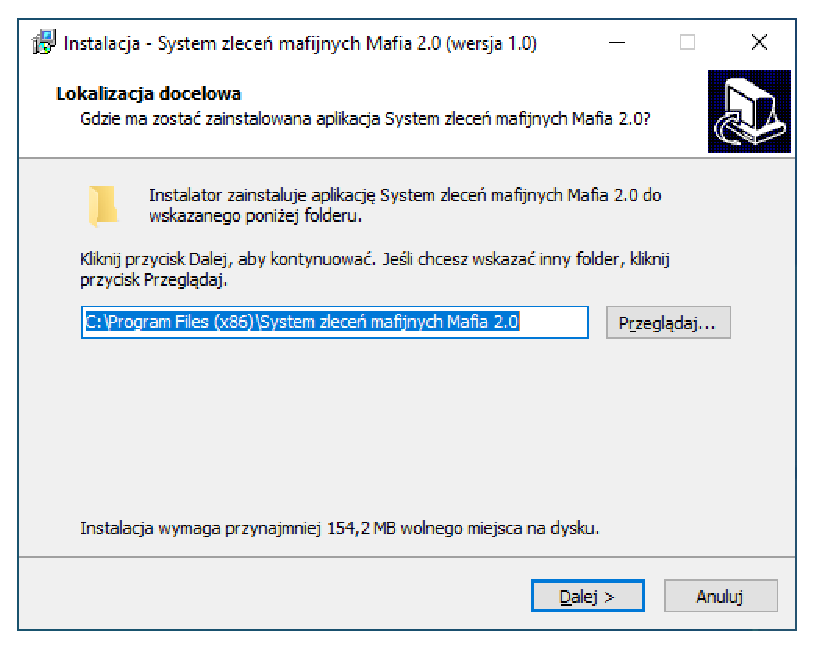
\includegraphics[width=8cm]{img/Local_Install_1.eps}
					\end{figure}


				%\end{figure}
				
				\item Po ukończeniu instalacji aplikacji, kreator zaproponuje instalację wymaganych do działania składników,
					\begin{figure}[H]
						\centering
						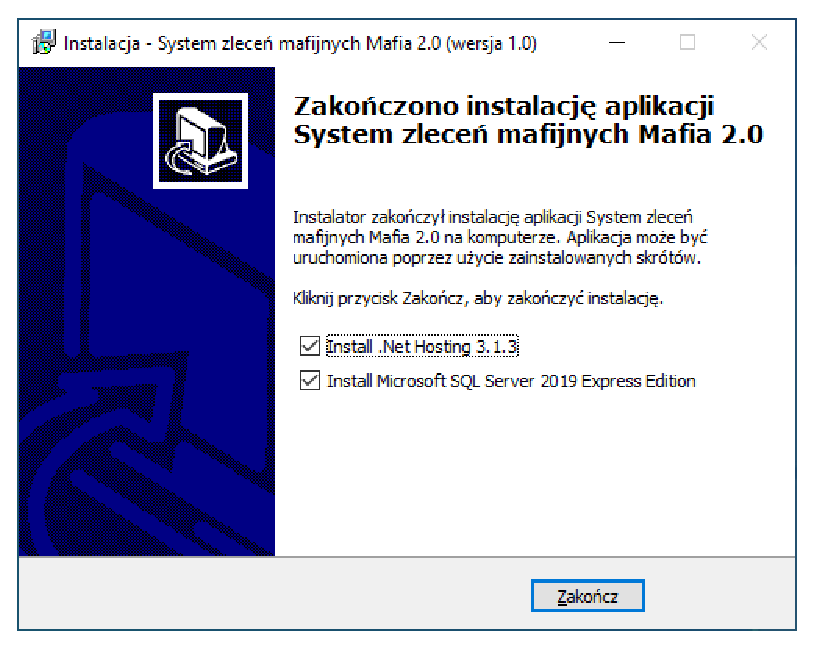
\includegraphics[width=8cm]{img/Local_Install_2.eps}
					\end{figure}		
					
				\item Zainstalować ASP.NET Core Runtime 3.1.3 Hosting Bundle (można pominąć jeśli jest już zainstalowane),
					\begin{figure}[H]
						\centering
						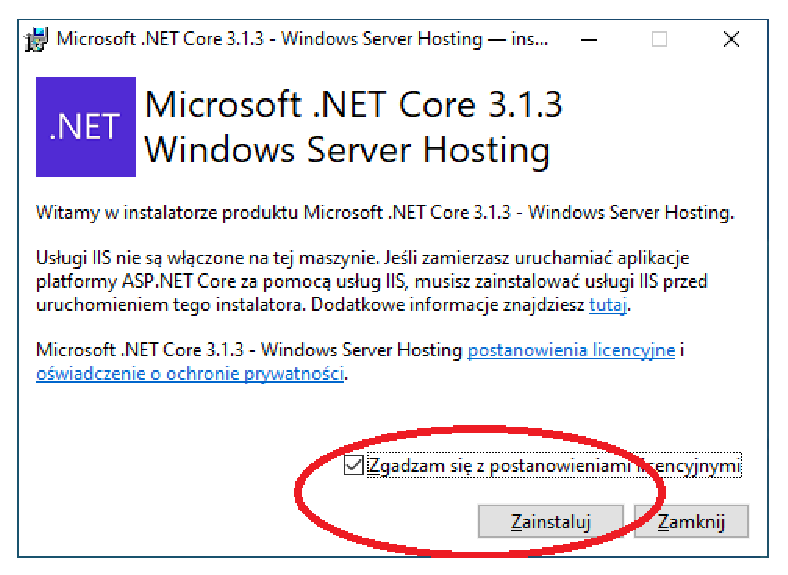
\includegraphics[width=8cm]{img/Local_Install_3.eps}
					\end{figure}
					
				\item Zainstalować Microsoft SQL Server 2019 Express Edition, wybierając wersję instalacji: ,,Basic'' (można pominąć jeśli jest już zainstalowane),
					\begin{figure}[H]
						\centering
						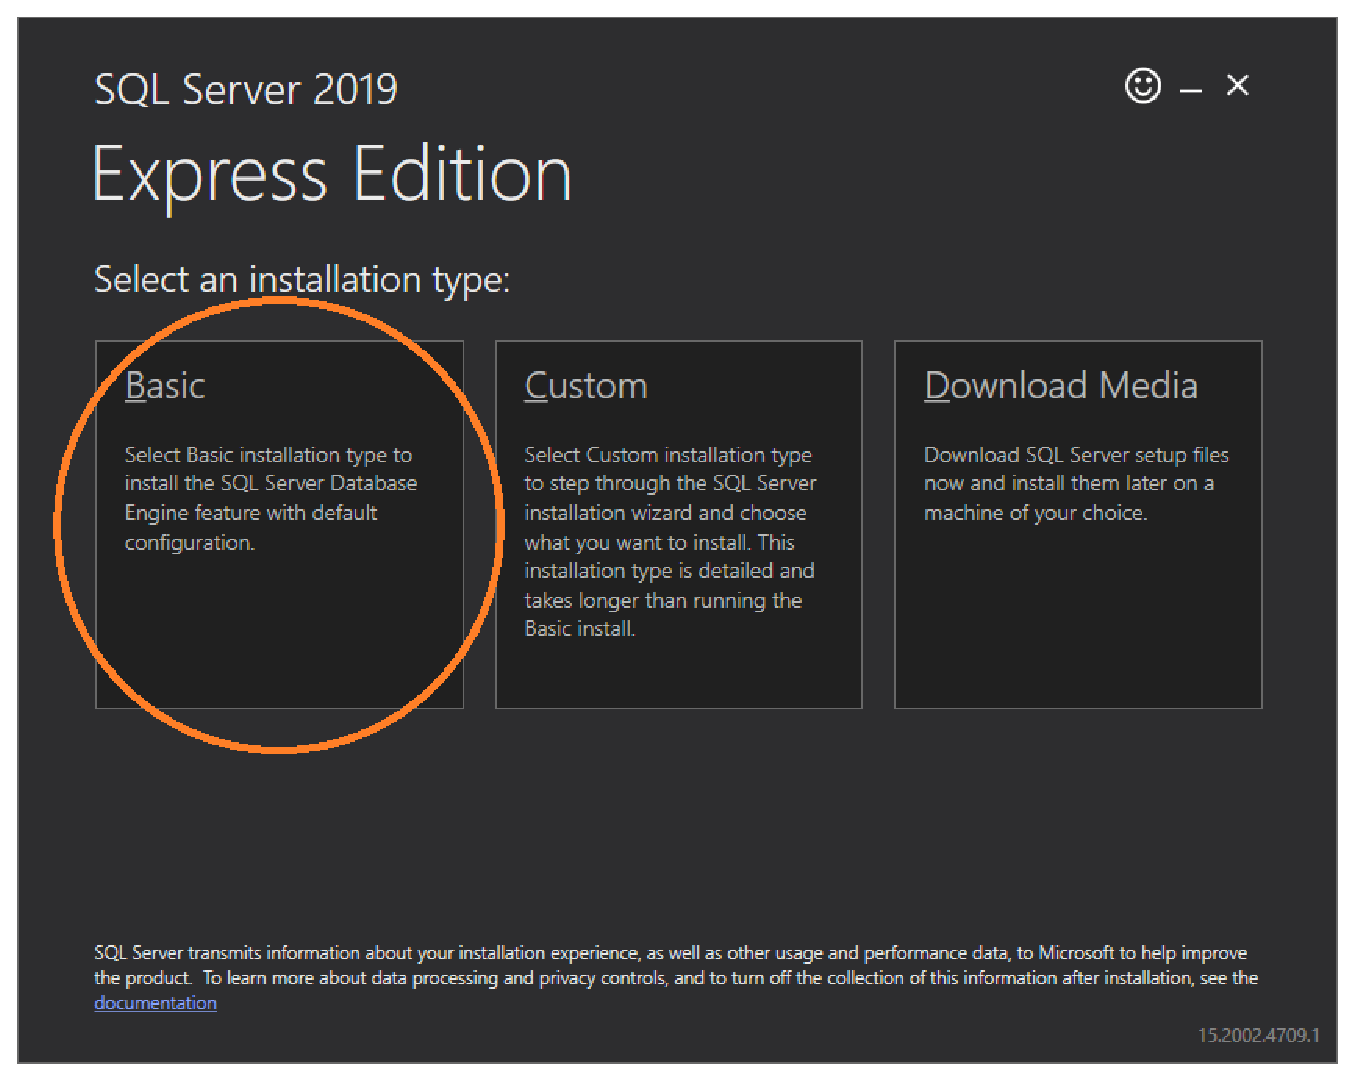
\includegraphics[width=8cm]{img/Local_Install_4.eps}
					\end{figure}
					
				\item Po zakończeniu instalacji serwera SQL, można przejść do strony pobierania aplikacji SQL Server Management Studio (1. Install SSMS) albo zakończyć działanie
					instalatora (2. Close)
					\begin{figure}[H]
						\centering
						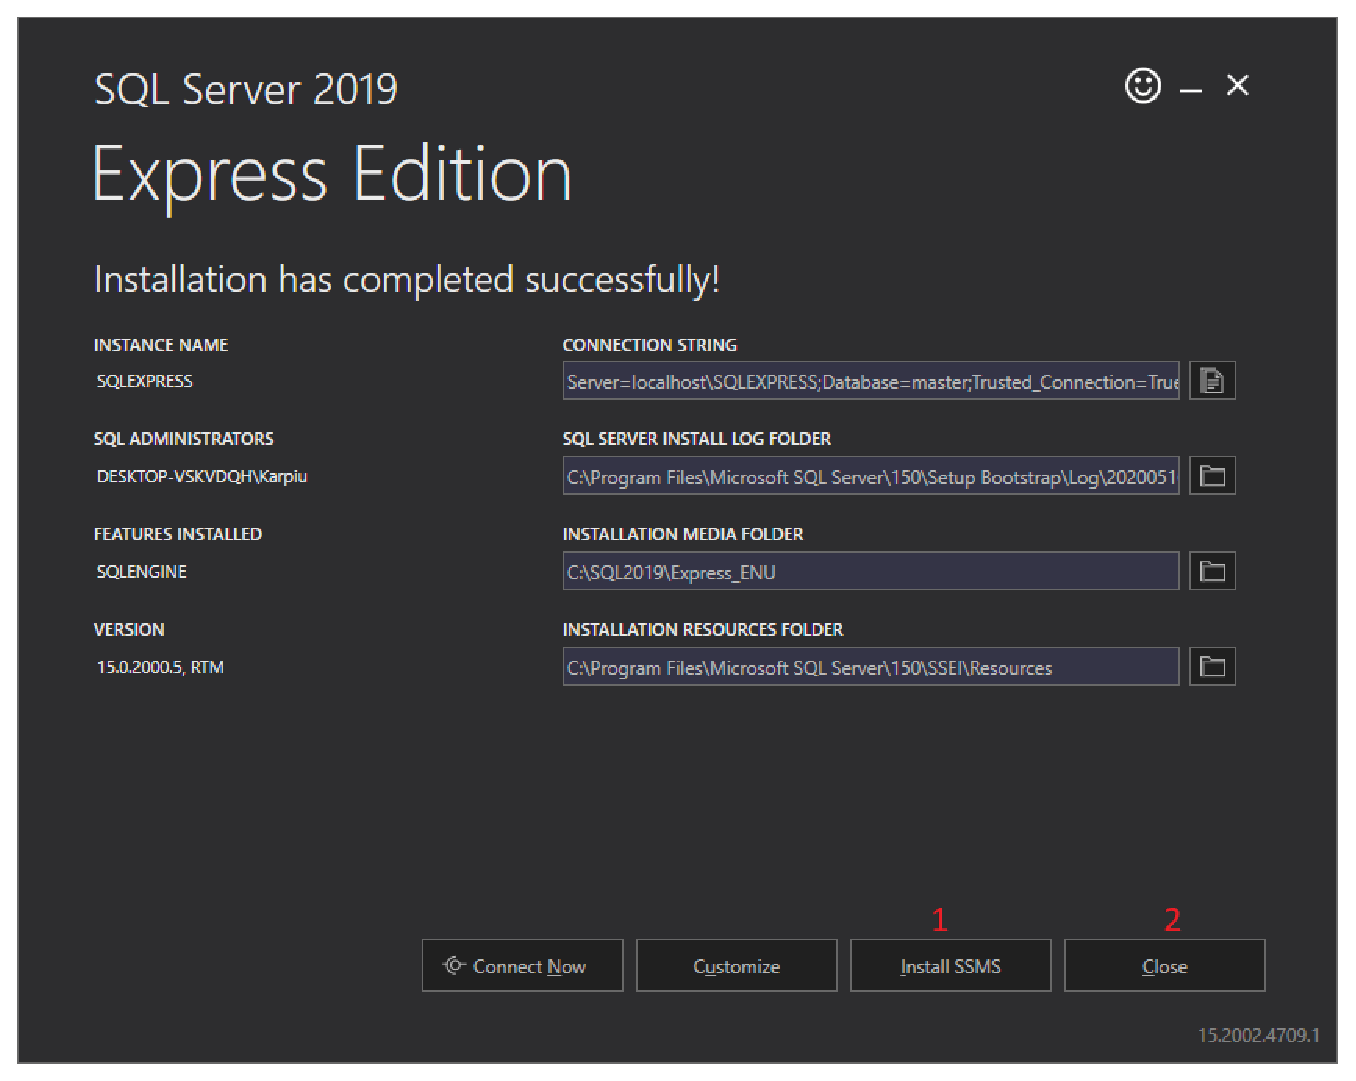
\includegraphics[width=8cm]{img/Local_Install_5.eps}
					\end{figure}		
							
				\item Pobrać ze strony internetowej instalator SQL Server Management Studio (SSMS),
					\begin{tcolorbox}[minipage,colback=white,arc=0pt,outer arc=0pt, fontupper=\footnotesize]
						\url{https://docs.microsoft.com/en-us/sql/ssms/download-sql-server-management-studio-ssms}
					\end{tcolorbox}
					\begin{figure}[H]
						\centering
						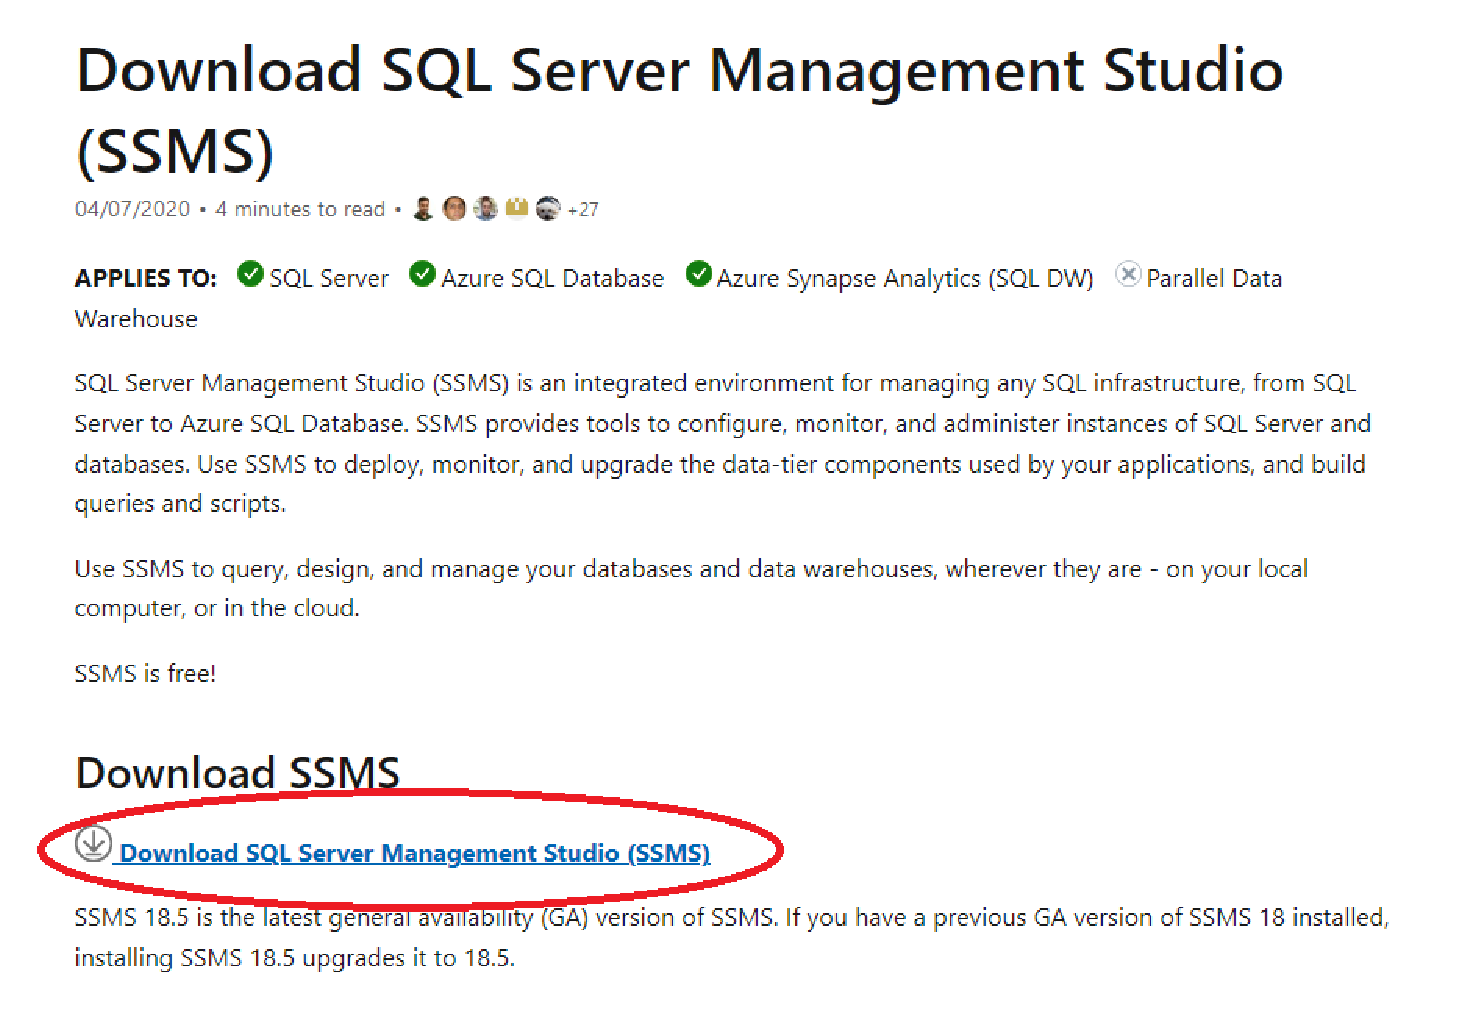
\includegraphics[width=8cm]{img/Local_Install_5.5.eps}
					\end{figure}
									
				\item Uruchomić pobrany plik i zainstalować SQL Server Management Studio,
					\begin{figure}[H]
						\centering
						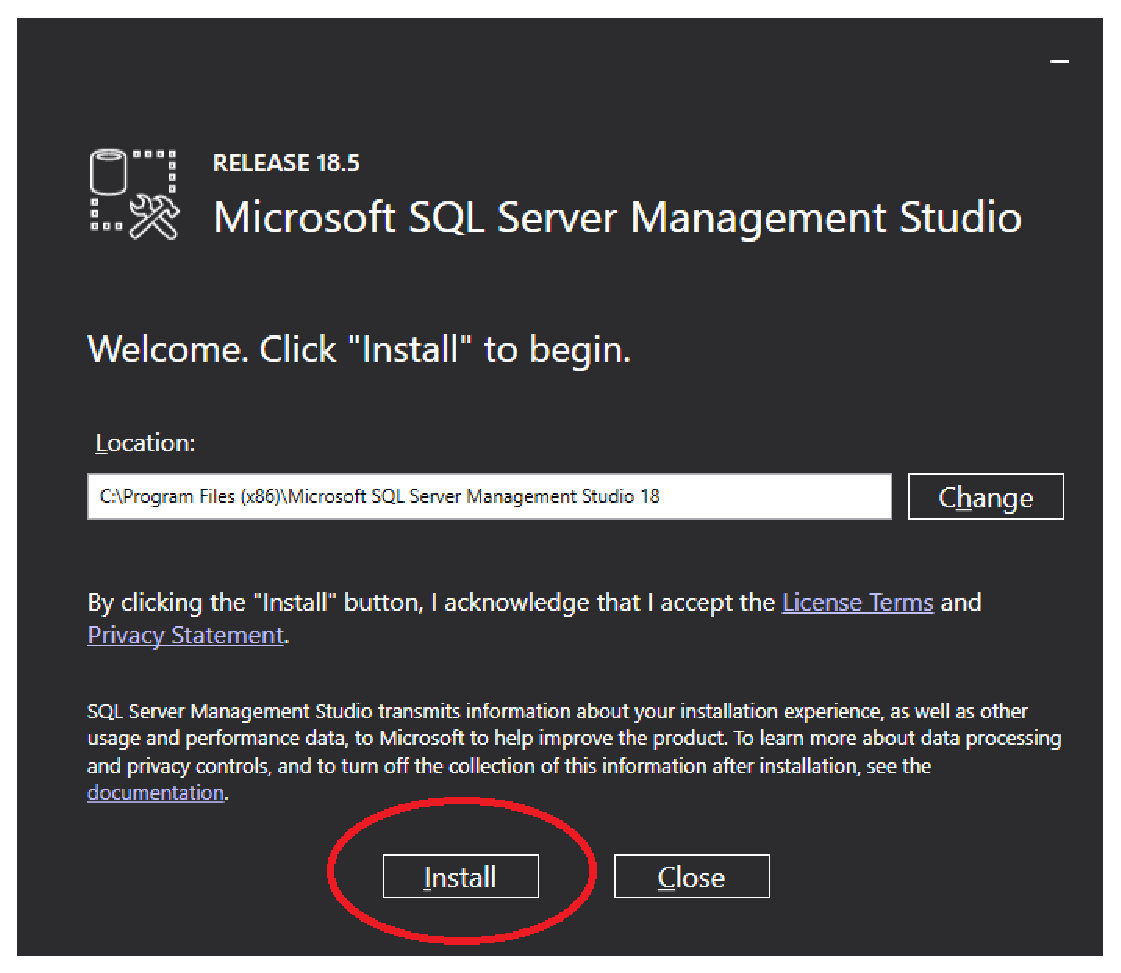
\includegraphics[width=8cm]{img/Local_Install_6.eps}
					\end{figure}
					
				\item Po ukończeniu instalacji SQL Server Management Studio należy uruchomić ponownie system,
					\begin{figure}[H]
						\centering
						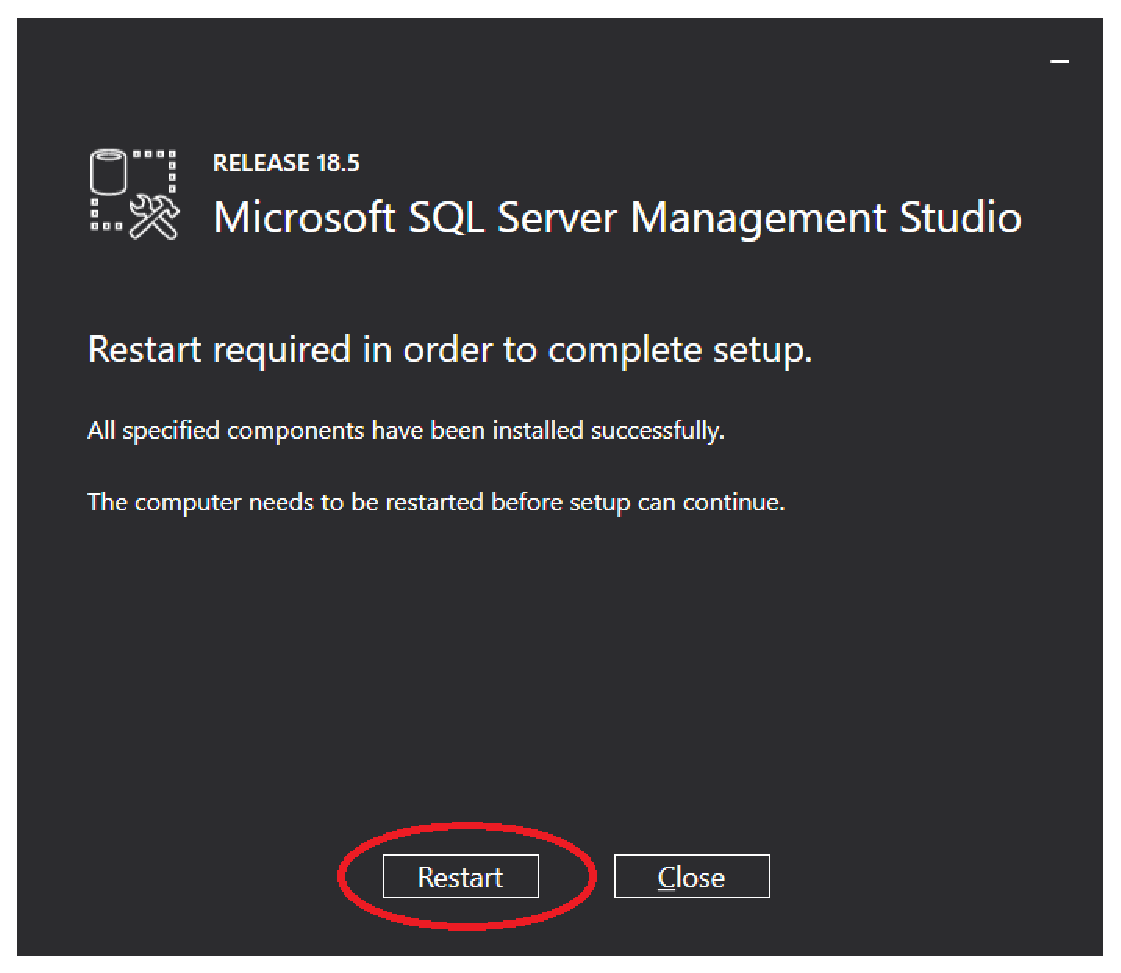
\includegraphics[width=8cm]{img/Local_Install_7.eps}
					\end{figure}
					
				\item Z menu ,,Start'' Uruchomić Microsoft SQL Server Management Studio 18,
					\begin{figure}[H]
						\centering
						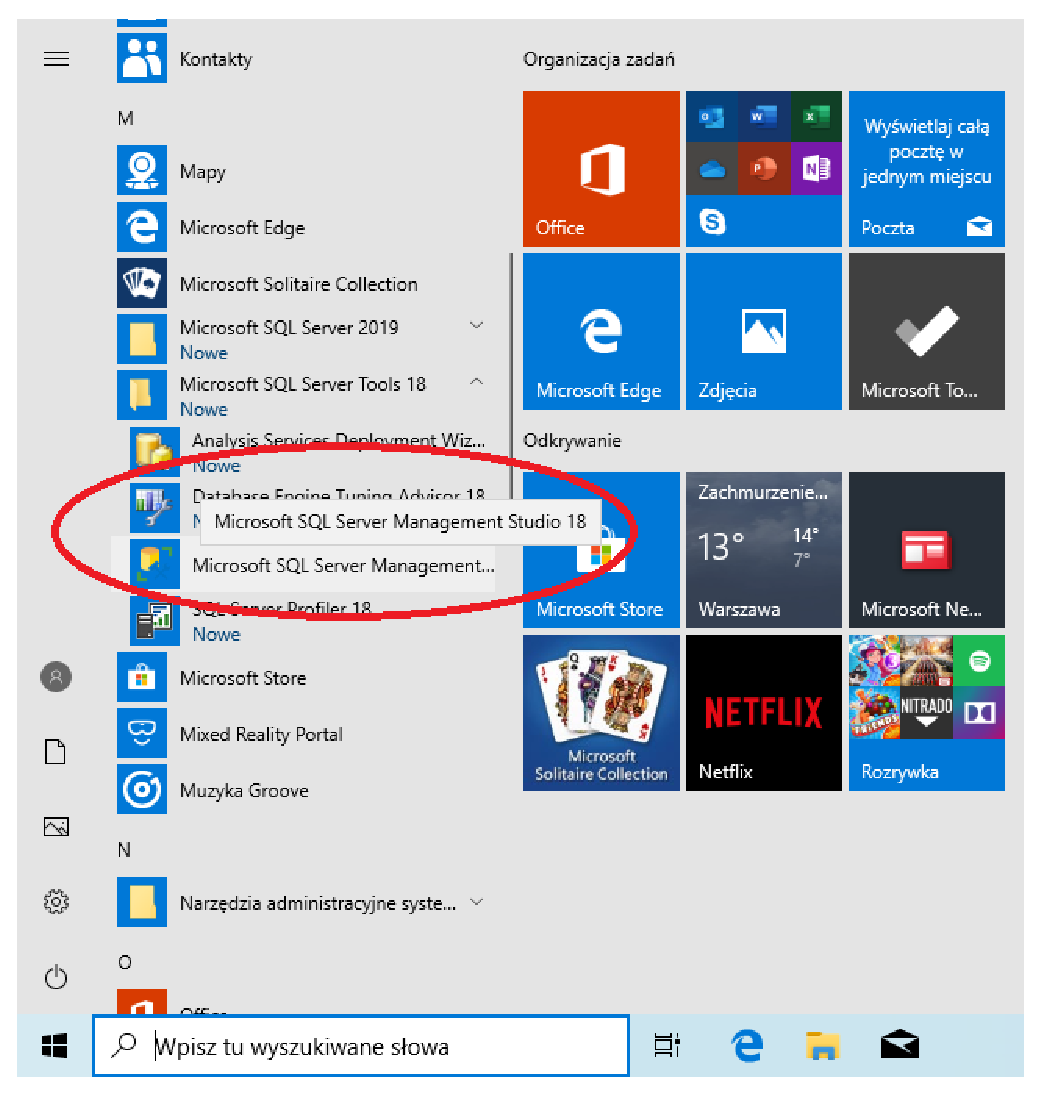
\includegraphics[width=8cm]{img/Local_Install_8.eps}
					\end{figure}
							
				\item Połączyć się z lokalną bazą danych,~
					\begin{figure}[H]
						\centering
						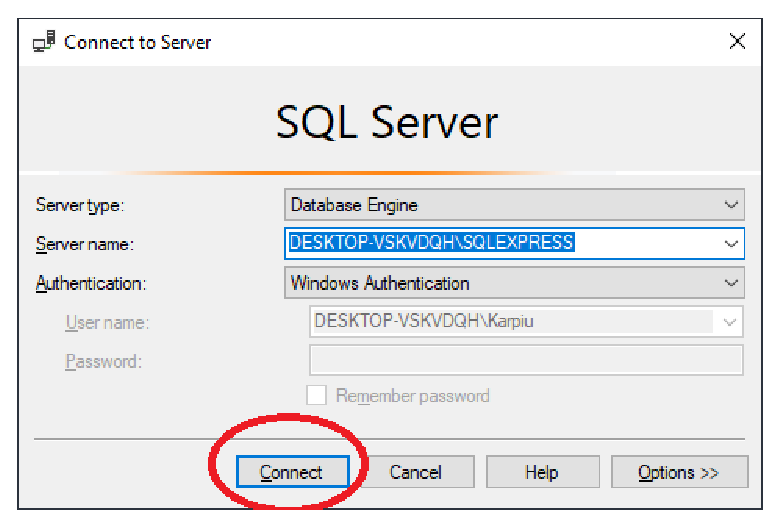
\includegraphics[width=8cm]{img/Local_Install_9.eps}
					\end{figure}
						
				\item Po podłączeniu do bazy danych należy rozwinąć listę składników bazy danych a następnie przy pomocy prawego przycisku myszy należy wybrać pole ,,Databases'' i wybrać
					Restore Database...''
					\begin{figure}[H]
						\centering
						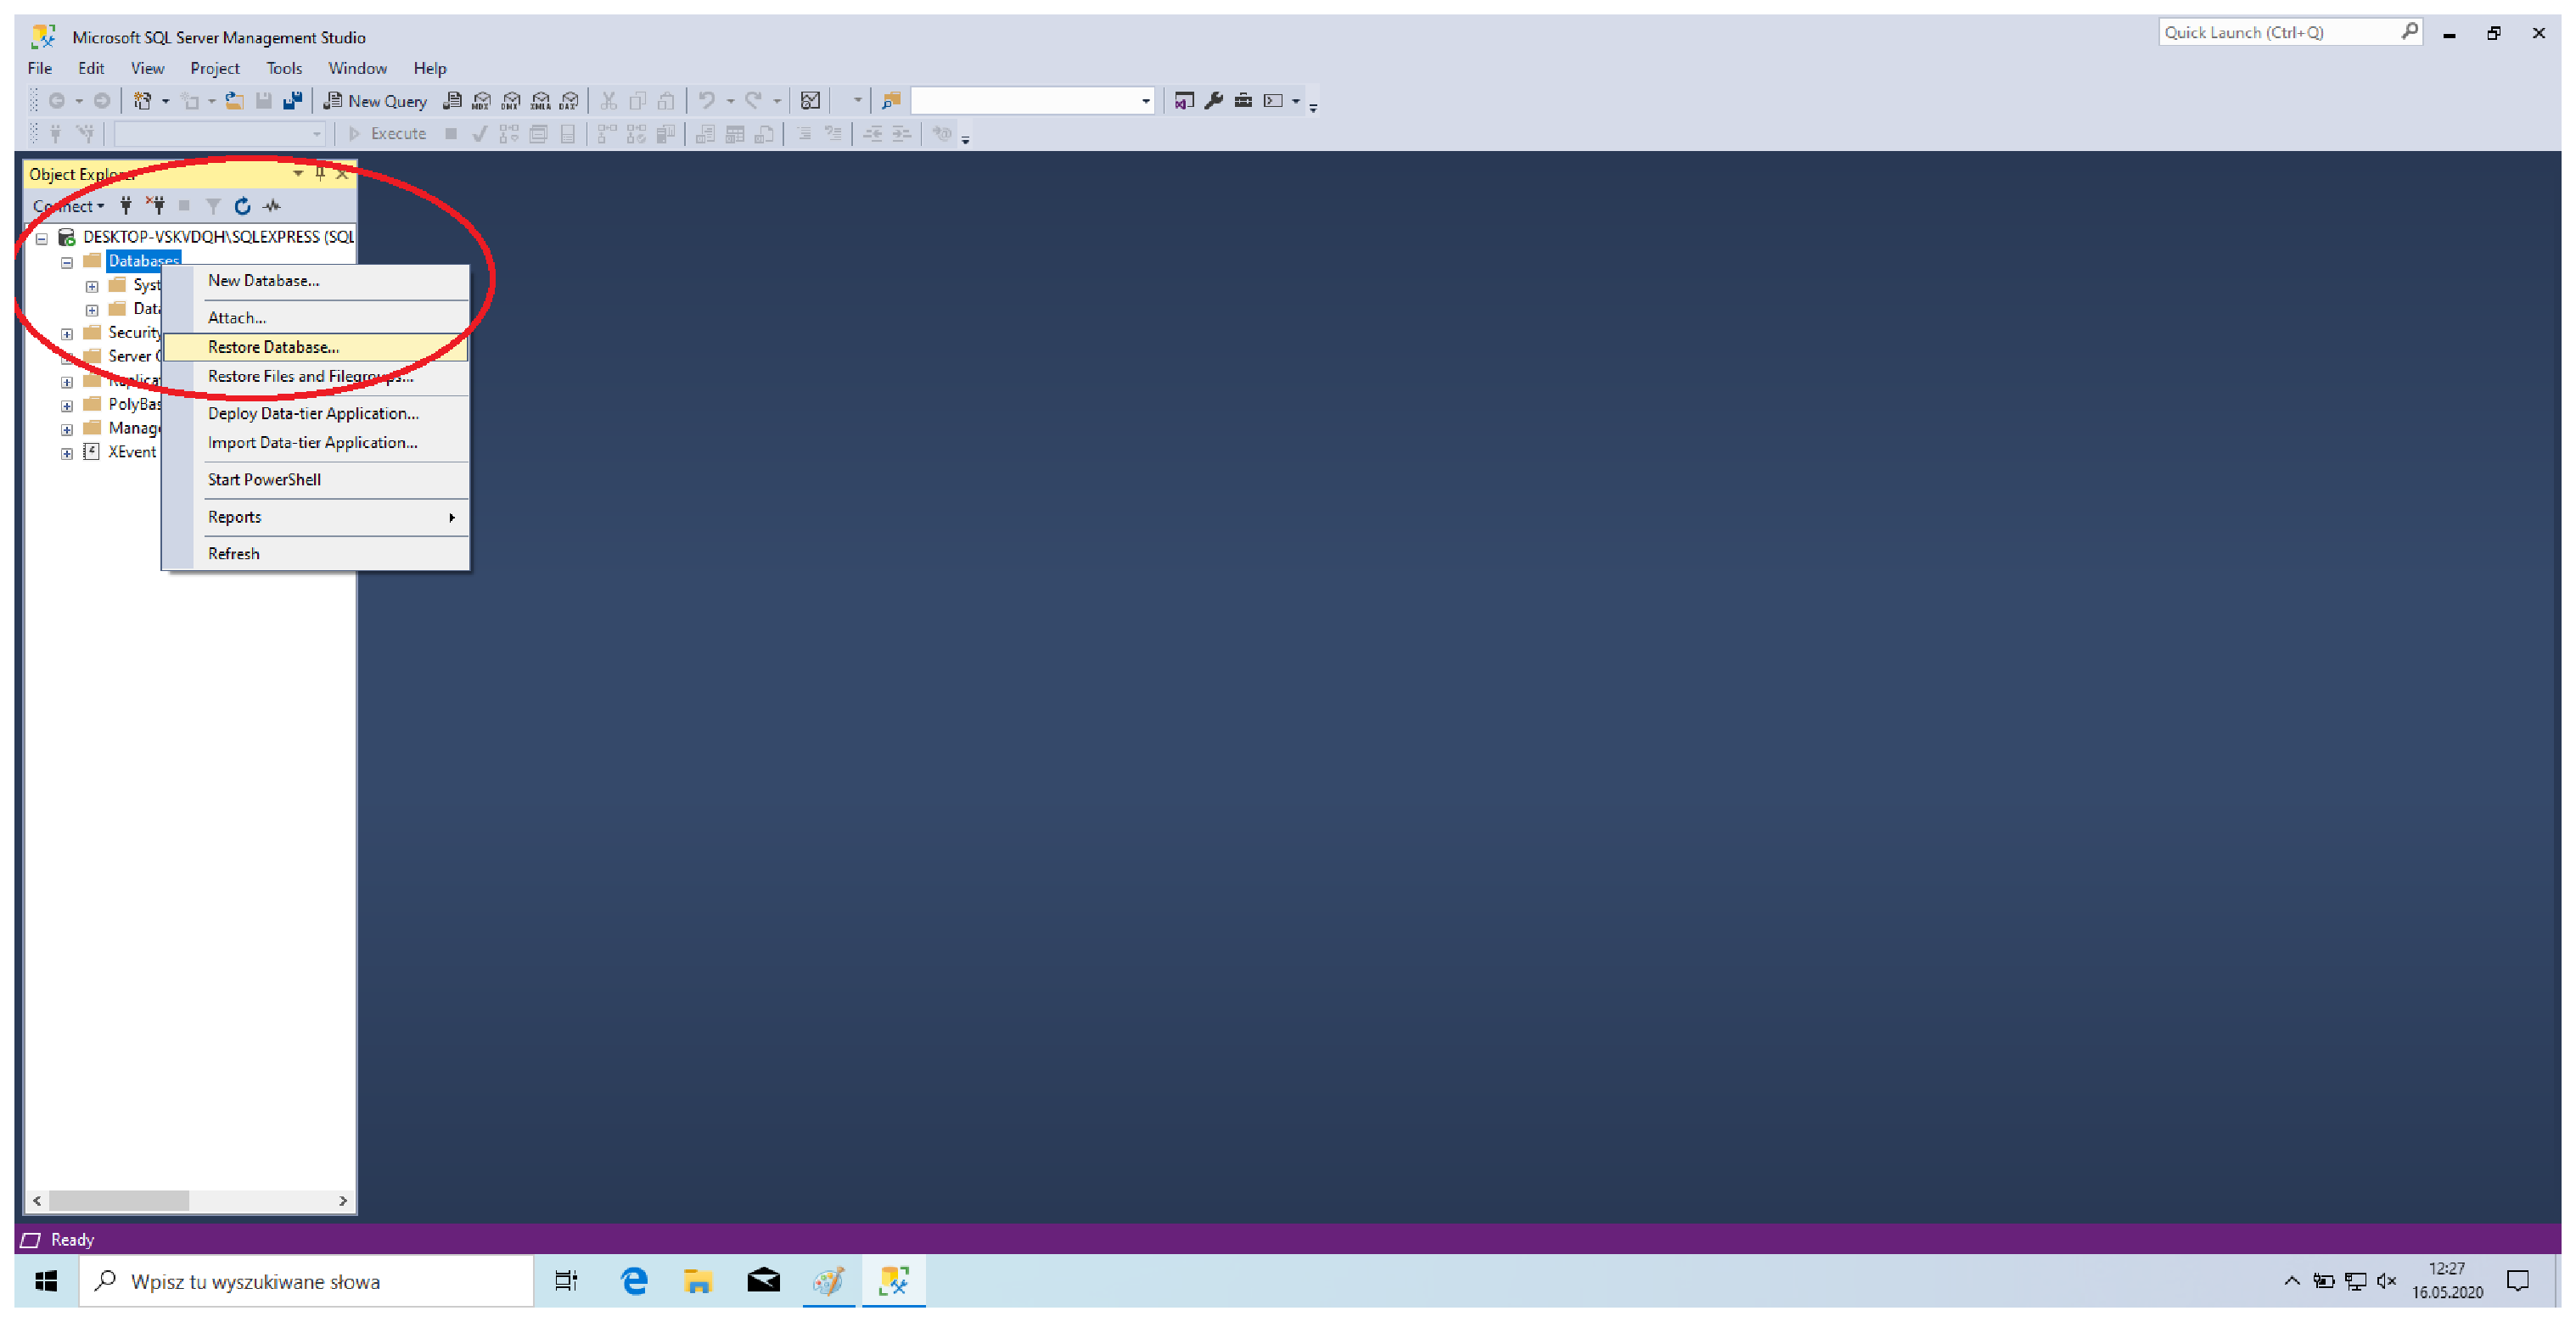
\includegraphics[width=8cm]{img/Local_Install_10.eps}
					\end{figure}
									 					
				\item Przywrócić bazę danych z pliku o nazwie ,,PAM\_KillersDB.bak'' znajdującego się na lokalnym dysku ,,C:$\backslash$'',
					\begin{figure}[H]
						\centering
						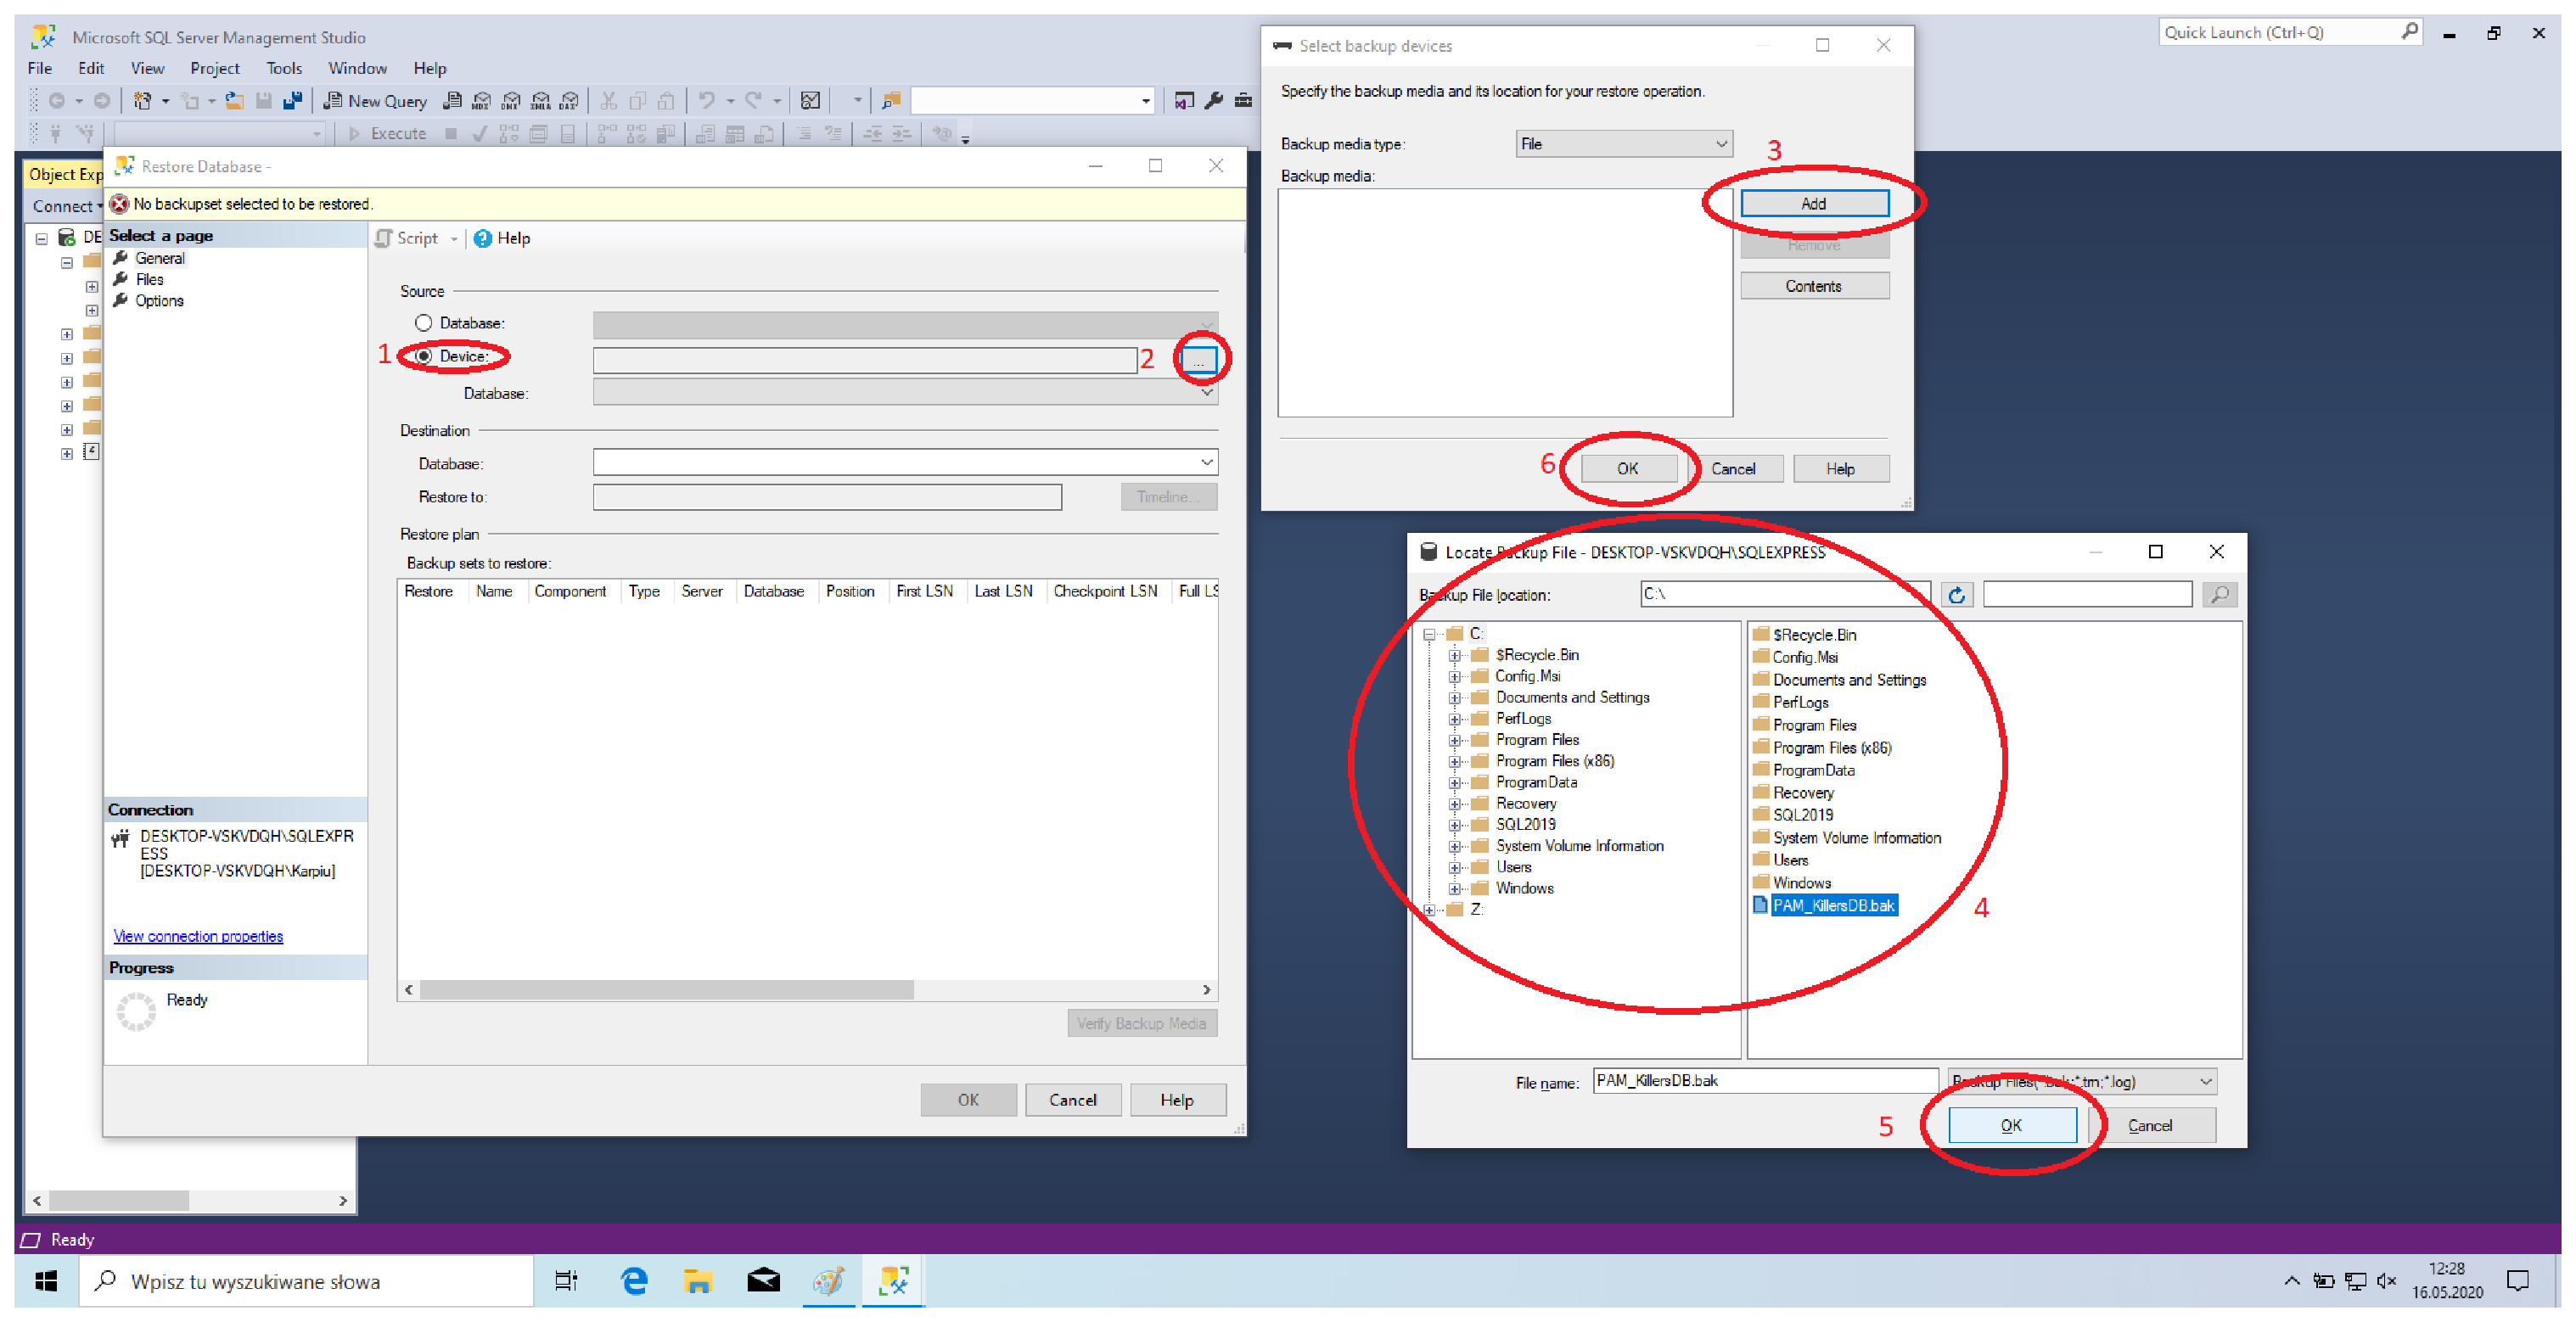
\includegraphics[width=8cm]{img/Local_Install_11.eps}\\
						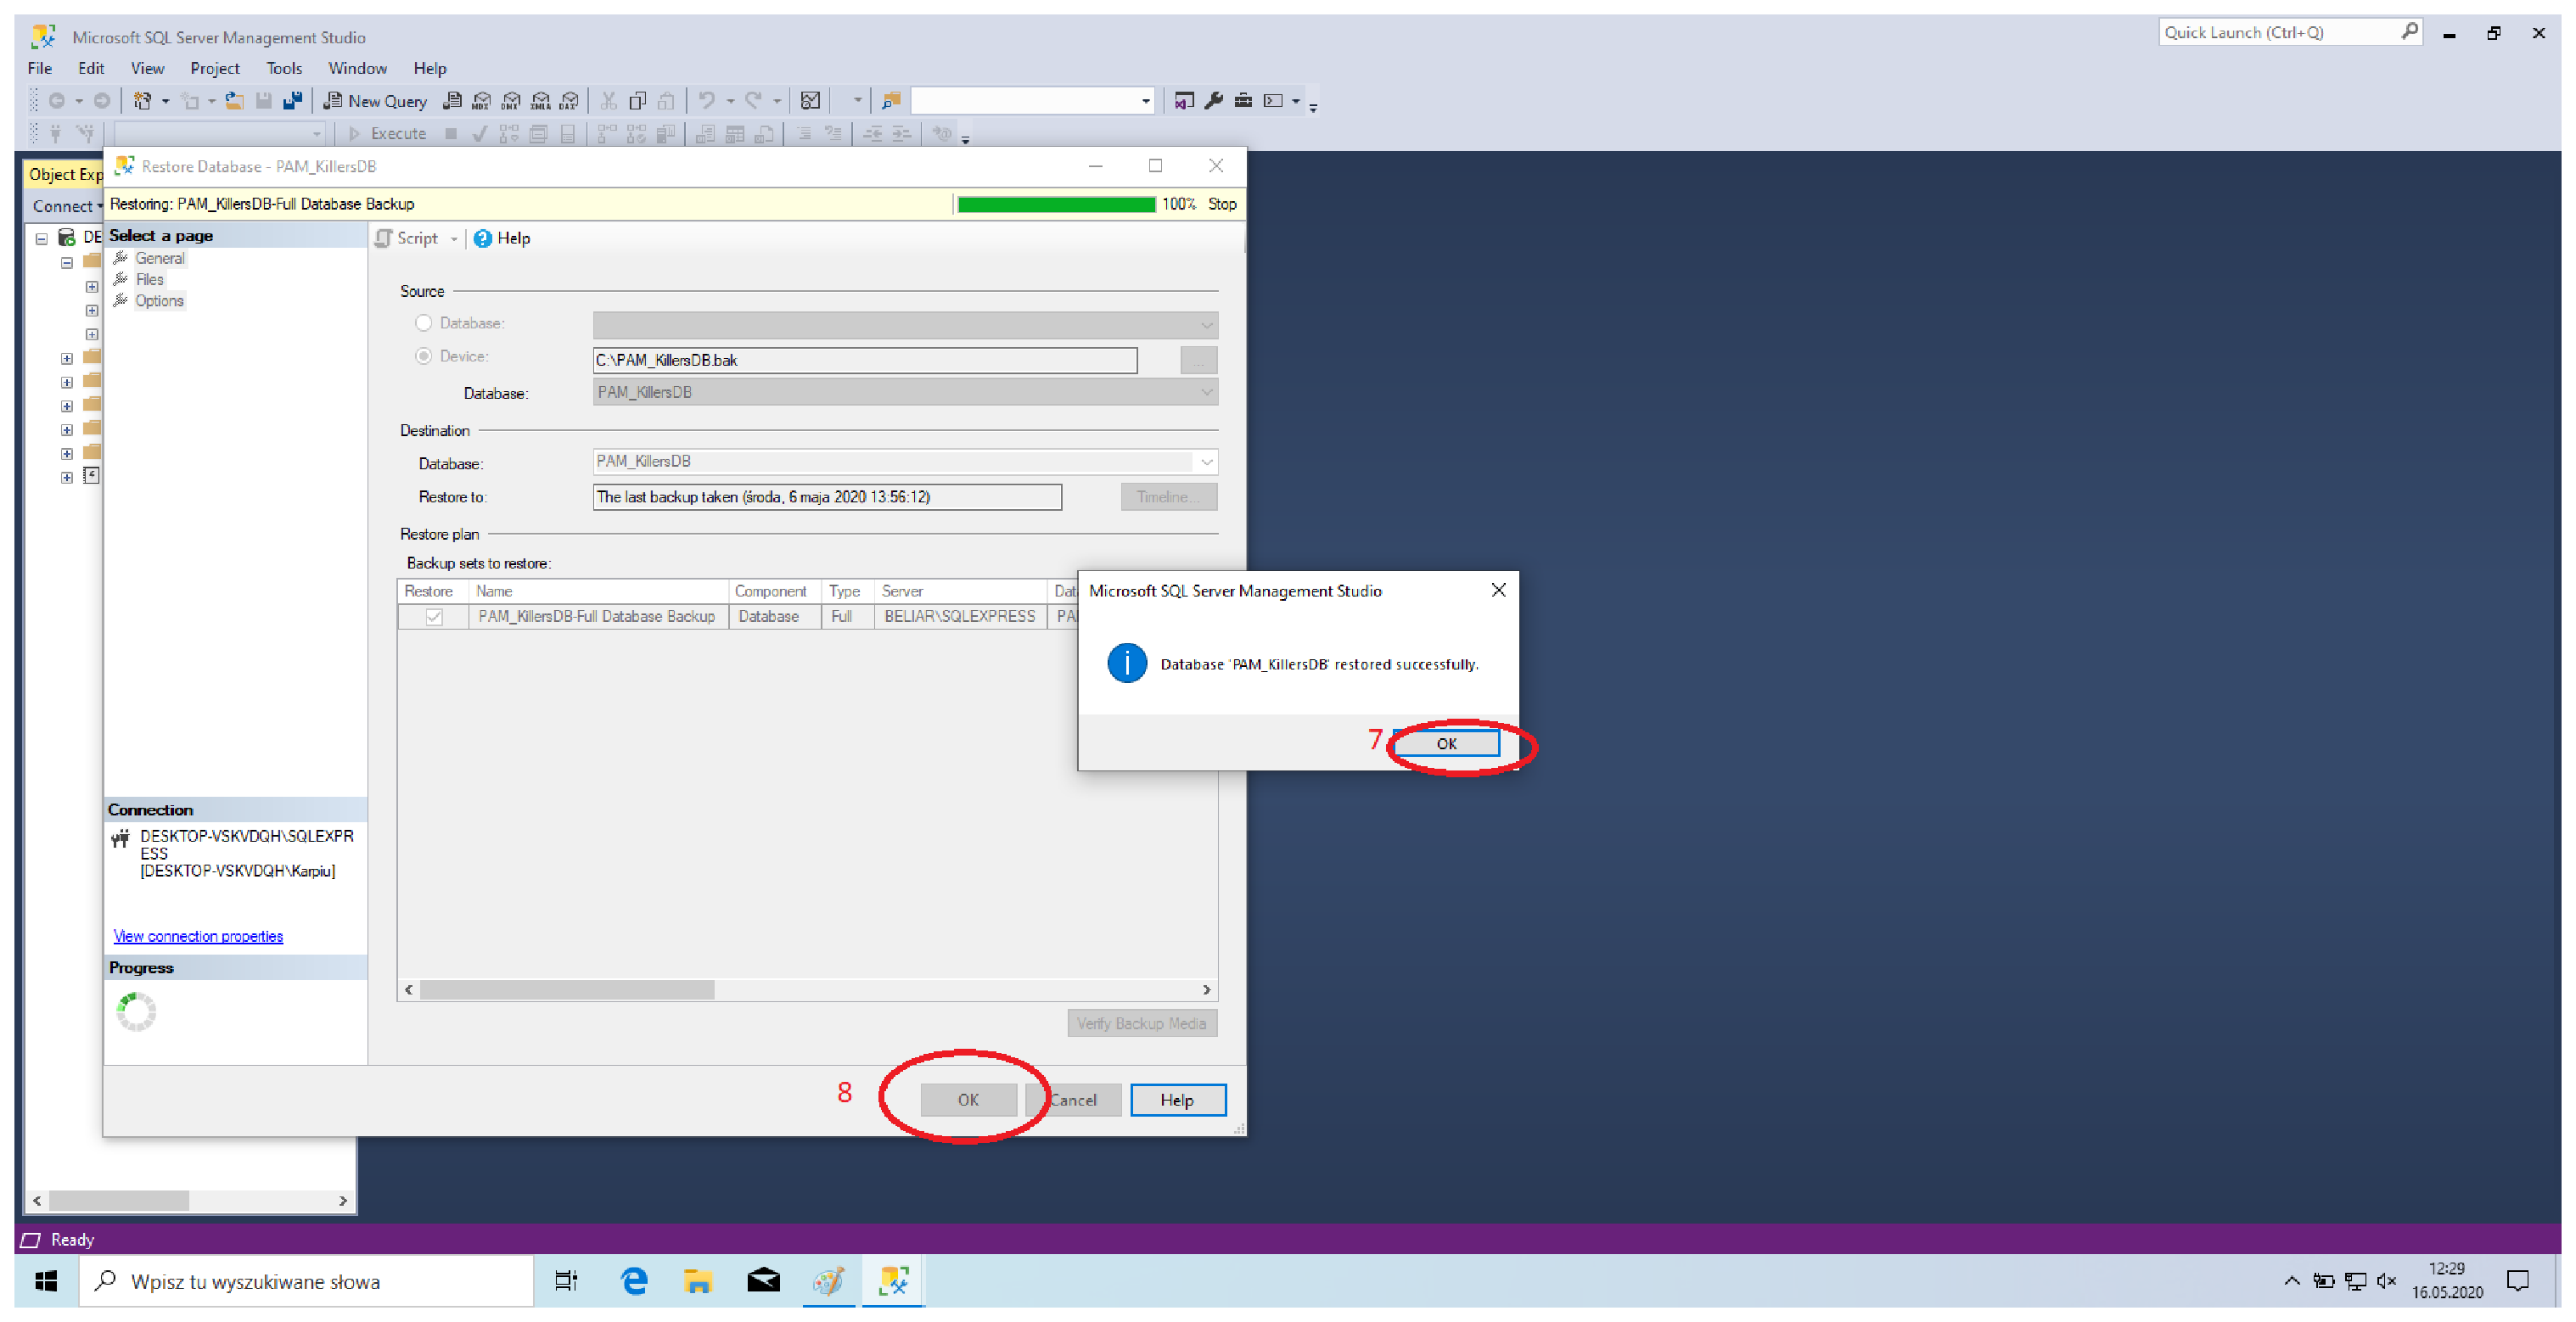
\includegraphics[width=8cm]{img/Local_Install_12.eps}
					\end{figure}
									
				\item Przy pomocy aplikacji ,,Notatnik'' należy edytować plik ,,appsettings.json'' znajdujący się w głównym katalogu aplikacji (Domyślnie:
					,,C:$\backslash$Program Files$\backslash$System zleceń mafijnych Mafia 2.0'') i zmienić wartości w sekcji ,,EmailConfiguration'', zgodnie z ustawieniami podanymi
					przez administratora serwera pocztowego,
					\begin{figure}[H]
						\centering
						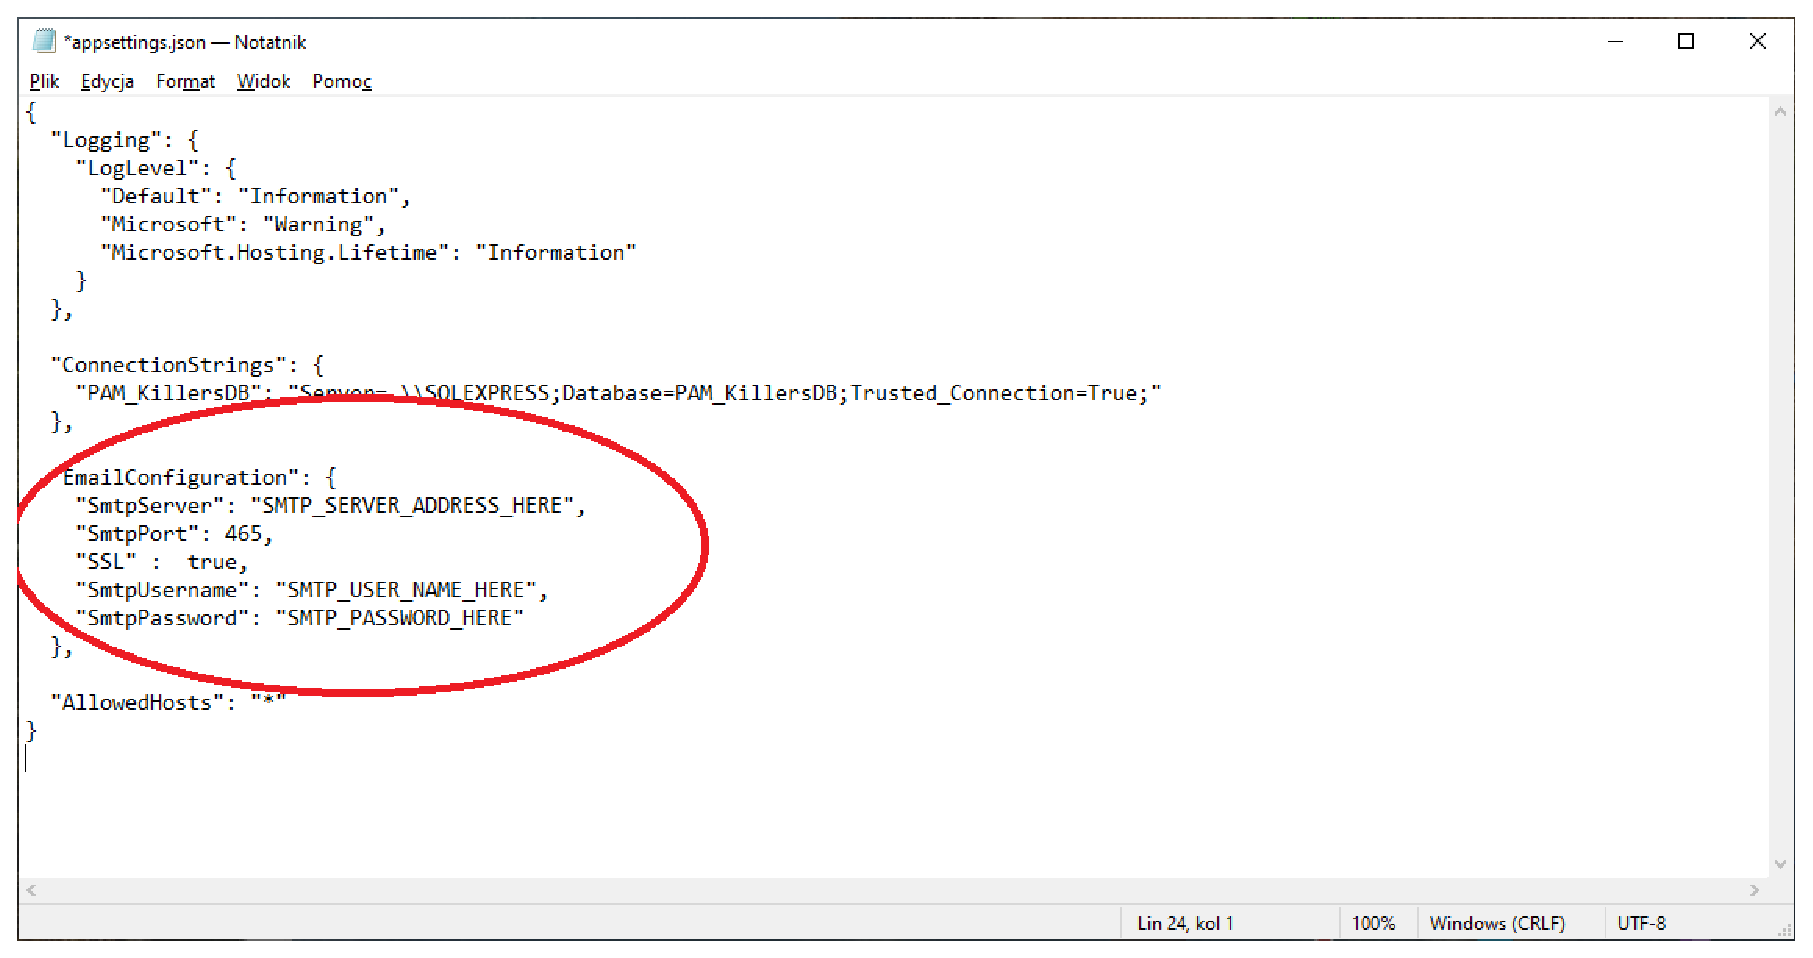
\includegraphics[width=8cm]{img/Local_Install_13.eps}
					\end{figure}				
					
				\item Uruchomić ponownie system.
			\end{enumerate}
			System zleceń mafijnych ,,Mafia 2.0'' jest gotowy do używania na lokalnym komputerze. Aby uruchomić aplikację należy użyć skrótu w menu ,,Start'', na Pulpicie (jeżeli została
			zaznaczona odpowiednia opcja w czasie instalacji) lub przy pomocy przeglądarki internetowej udać się pod adres:
			\begin{tcolorbox}[minipage,colback=white,arc=0pt,outer arc=0pt, fontupper=\footnotesize]
				\url {http://localhost:5000}
			\end{tcolorbox}
			\noindent W zależności od mocy obliczeniowej używanego komputera pierwsze uruchomienie aplikacji po starcie systemu operacyjnego może trwać dłużej.		
		
		\subsection{Zdalne uruchomienie systemu}
			\indent Do uruchomienia Systemu zleceń mafijnych Mafia 2.0 wymagane jest następujące oprogramowanie:
			\begin{itemize}
				\item Linux Ubuntu 18.04 LTS 64bit.
				\item apt-transport-https
				\item aspnetcore-runtime-3.1
				\item mssql-server
				\item msqsql-tools
				\item unixodbc-dev
				\item nginx
			\end{itemize}
			
			\begin{enumerate}
				\item Po wydaniu polecenia:
					\begin{tcolorbox}[minipage,colback=white,arc=0pt,outer arc=0pt, fontupper=\scriptsize]
						wget -O - https://github.com/Karpfly2822/Test-VS-Repo/releases/download/1/PAM\_Linux\_Installer.sh $|$ bash
					\end{tcolorbox}			
					nastąpi pobranie i instalacja wszystkich(oprócz Ubuntu) wymaganych pakietów oraz samej aplikacji systemu zleceń.
			
				\item Po zakończeniu skryptu należy przeprowadzić konfigurację bazy danych MSSQL:
					\begin{tcolorbox}[minipage,colback=white,arc=0pt,outer arc=0pt, fontupper=\footnotesize]			
						sudo /opt/mssql/bin/mssql-conf setup
					\end{tcolorbox}
					Gdzie należy podać hasło, wybrać typ instalacji (3 Express) i język użytkownika.
					
				\item Po zakończeniu konfiguracji należy połączyć się z serwerem bazy danych i przywrócić bazę z pliku
					PAM\_KillersDB.bak znajdującego się w ,,/var/opt/mssql/backup/''.	
					\begin{tcolorbox}[minipage,colback=white,arc=0pt,outer arc=0pt, fontupper=\footnotesize]			
						/opt/mssql-tools/bin/sqlcmd -S localhost -U SA \\
						RESTORE DATABASE PAM\_KillersDB	\\
						FROM DISK = '/var/opt/mssql/backup/PAM\_KillersDB.bak'	\\
						WITH MOVE 'PAM\_KillersDB' TO '/var/opt/mssql/data/PAM\_KillersDB.mdf',	\\
						MOVE 'PAM\_KillersDB\_Log' TO '/var/opt/mssql/data/PAM\_KillersDB\_Log.ldf'	\\
						GO \\
						EXIT
					\end{tcolorbox}				
			
				\item Konfiguracja NGINX:
					przy pomocy edytora tekstu należy otworzyć plik:
					\begin{tcolorbox}[minipage,colback=white,arc=0pt,outer arc=0pt, fontupper=\footnotesize]
						sudo vim /etc/nginx/sites-available/default
					\end{tcolorbox}	
					oraz zastąpić domyślną konfigurację następującą:
					\begin{tcolorbox}[minipage,colback=white,arc=0pt,outer arc=0pt, fontupper=\footnotesize]
						\begin{tabbing}
							ser\= ver \{\\
								\> listen	80;\\
    							\> server\_name   example.com *.example.com;\\
    							\> loc\= ation / \{\\
        						\>\> proxy\_pass         http://localhost:5000;\\
        						\>\> proxy\_http\_version 1.1;\\
        						\>\> proxy\_set\_header   Upgrade \$http\_upgrade;\\
        						\>\> proxy\_set\_header   Connection keep-alive;\\
        						\>\> proxy\_set\_header   Host \$host;\\
        						\>\> proxy\_cache\_bypass \$http\_upgrade;\\
        						\>\> proxy\_set\_header   X-Forwarded-For \$proxy\_add\_x\_forwarded\_for;\\
        						\>\> proxy\_set\_header   X-Forwarded-Proto \$scheme;\\
        						\>\> gzip on;\\
        						\>\> gzip\_types text/plain application/xml text/css application/javascript;\\
        						\>\> gzip\_min\_length 1000;\\
		    					\> \}\\
							\}
						\end{tabbing}
					\end{tcolorbox}				
			
				\item po zapisaniu konfiguracji NGINX należy sprawdzić za pomocą polecenia poprawność konfiguracji:
					\begin{tcolorbox}[minipage,colback=white,arc=0pt,outer arc=0pt, fontupper=\footnotesize]
						sudo nginx -t
					\end{tcolorbox}
		
				\item jeżeli test konfiguracji przeszedł pozytywnie należy przeładować NGINX z nowymi ustawieniami:	
					\begin{tcolorbox}[minipage,colback=white,arc=0pt,outer arc=0pt, fontupper=\footnotesize]
						sudo nginx -s reload
					\end{tcolorbox}			
			
				\item przy pomocy edytora tekstu należy otworzyć plik:
					\begin{tcolorbox}[minipage,colback=white,arc=0pt,outer arc=0pt, fontupper=\footnotesize]
						sudo vim /var/www/PAM/appsettings.json
					\end{tcolorbox}						
					W polu ,,Password='' należy wprowadzić hasło do serwera bazy danych, następnie w~sekcji ,,EmailConfiguration'' należy podać dane serwera e-mail.
				\item Po zapisaniu pliku należy zrestartować aplikację przy pomocy polecenia:
					\begin{tcolorbox}[minipage,colback=white,arc=0pt,outer arc=0pt, fontupper=\footnotesize]
						sudo systemctl restart PAM
					\end{tcolorbox}
				\item Aby aplikacja była dostępna poprzez sieć internet należy przekierować port 80 w konfiguracji routera (wartość ,,listen 80'' w konfiguracji NGINX).
				\item Od tej chwili aplikacja będzie dostępna z dowolnej przeglądarki internetowej, poprzez udanie się pod adres ip lub domenę serwera. 
			\end{enumerate}
	\newpage
	
	\section{Wnioski projektowe}
		\indent Tworzenie aplikacji internetowej systemu zleceń mafijnych ,,Mafia 2.0'' było bardzo ciekawym doświadczaniem, w którym zdobyliśmy wiele praktycznej wiedzy jak w poprawny sposób
		stworzyć profesjonalną aplikację internetową począwszy od wyboru wykorzystywanej technologi, poprzez projekt frontendu i funkcjonalności backendu oraz napisanie dokumentacji
		w \LaTeX \space	- co jak się okazało nie było takie trudne jak na pierwszy rzut oka mogło by się wydawać. Wdrożenie aplikacji internetowej opartej o framework
		ASP.NET Core 3.1 okazało się o wiele prostsze na systemie Linux przy wykorzystaniu reverse proxy NGINX, niż w~systemie Windows Server przy użyciu IIS.
		Praca w grupie wykazała że każdy z nas posiada inny zestaw umiejętności i wiedzy dzięki czemu w naturalny sposób wytworzył się podział prac przy projekcie,
		jednocześnie gdy napotykany był jakiś problem to różnice w~posiadanej wiedzy pozwalały na wspólne szybkie rozwiązanie problemu. 		
\end{document}